\documentclass[aspectratio=169]{beamer}
\usepackage{color,amsmath}
\usepackage{subfigure}
\usepackage{booktabs}
\usepackage{framed}
\usepackage{comment}

\def\vf{\vfill}

%%%%%%%%%%%%%%%%%%%%%%%%%%
\title[]{3Rs: Replace, Refine, Reduce}
\author[]{Matthew J. Salganik\\Department of Sociology\\Princeton University}
\date[]{Summer Institute in Computational Social Science\\June 23, 2018
\vfill
\begin{flushleft}
{\scriptsize
The Summer Institute in Computational Social Science is supported by grants from the Russell Sage Foundation and the Alfred P. Sloan Foundation.}
\end{flushleft}
\begin{flushright}

\includegraphics[width=0.1\textwidth]{figures/cc-by.png}
\end{flushright}
}
\begin{document}
%%%%%%%%%%%%%%%%%%%%%%%%%%
\frame{\titlepage}
%%%%%%%%%%%%%%%%%%%%%%%%%%
\begin{frame}

\begin{center}

\includegraphics[width=0.5\textwidth]{figures/cute_kitten_kittenwar}
\end{center}

\vf
\tiny{\url{http://www.kittenwar.com/kittens/69827/}}

\end{frame}
%%%%%%%%%%%%%%%%%%%%%%%%%
\begin{frame}

\begin{center}
\Large{\textit{The Principles of Humane Experimental Technique}}\\
by Russell and Burch (1959)
\end{center}

\vf

\begin{itemize}
  \item \LARGE{Replace}
  \item \LARGE{Refine}
  \item \LARGE{Reduce}
\end{itemize}

\end{frame}
%%%%%%%%%%%%%%%%%%%%%%%%%
\begin{frame}

\begin{center}

\includegraphics[width=\textwidth]{figures/kramer_experimental_2014_title}
\end{center}

\vf
\tiny{\url{http://dx.doi.org/10.1073/pnas.1320040111}}

\end{frame}
%%%%%%%%%%%%%%%%%%%%%%%%%%%
\begin{frame}

\begin{center}
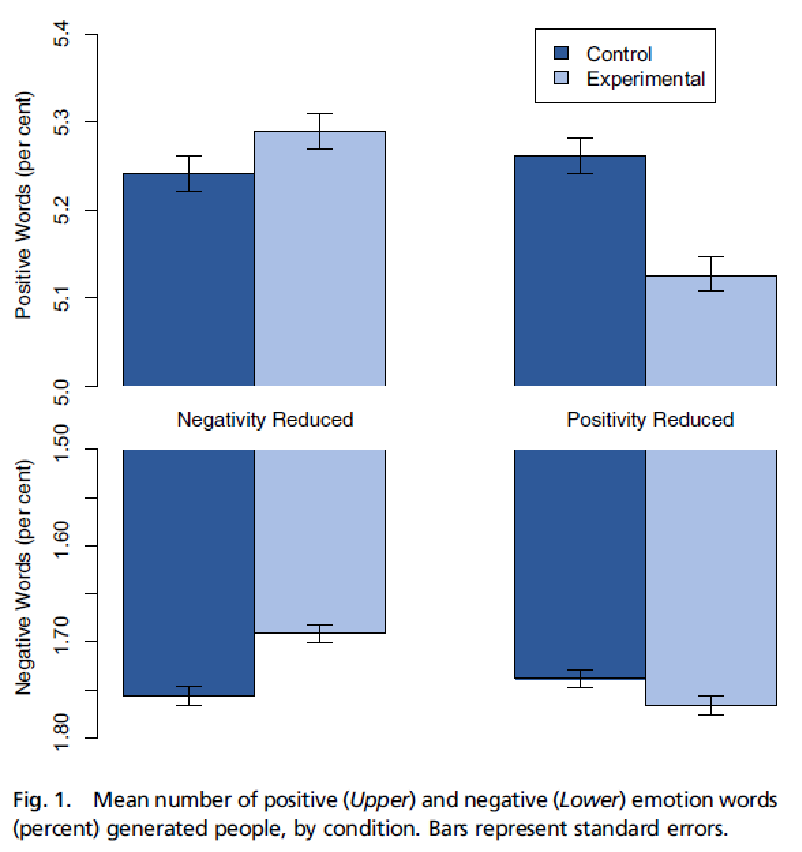
\includegraphics[width=0.5\textwidth]{figures/kramer_experimental_2014_fig1}
\end{center}

\end{frame}
%%%%%%%%%%%%%%%%%%%%%%%%%%%
\begin{frame}

\begin{center}

\includegraphics[width=0.8\textwidth]{figures/kramer_experimental_2014_concern}
\end{center}

\end{frame}
%%%%%%%%%%%%%%%%%%%%%%%%%%%
\begin{frame}

\begin{framed}
\textbf{Replace} experiments with less invasive methods
\end{framed}

\pause
\begin{center}

\includegraphics[width=\textwidth]{figures/coviello_detecting_2014_title}
\end{center}

\end{frame}
%%%%%%%%%%%%%%%%%%%%%%%%%%%
\begin{frame}

\begin{framed}
\textbf{Refine} treatments to make them less harmful
\end{framed}

\pause
Rather than blocking posts, they could have boosted posts

\end{frame}
%%%%%%%%%%%%%%%%%%%%%%%%%%%
\begin{frame}

\begin{framed}
\textbf{Reduce} the number of participants
\end{framed}

\pause
\begin{itemize}
\item Difference-in-difference estimator rather than a difference-of-means estimator.  
\pause
\item Would have cut the required sample size, perhaps by half (based on Deng et al. (2013) \& Xie and Aurisset (2016)).
\end{itemize}

\end{frame}
%%%%%%%%%%%%%%%%%%%%%%%%%%%
\begin{frame}

When should we care about reducing the number of participants?
\pause
\begin{enumerate}
\item uncertainty about whether the experiment will cause harm
\item participation was not voluntary
\end{enumerate}

\end{frame}
%%%%%%%%%%%%%%%%%%%%%%%%%%%
\begin{frame}

\begin{center}
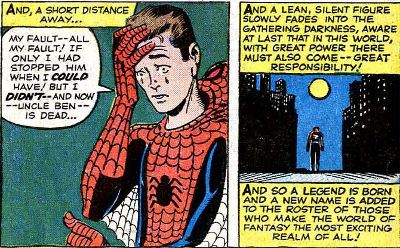
\includegraphics[width=0.7\textwidth]{figures/spiderman_great_power}
\end{center}

\pause

\LARGE{
\begin{center}
With great power there must also come\\great responsibility
\end{center}
}

\end{frame}
%%%%%%%%%%%%%%%%%%%%%%%%%%%%
\begin{frame}

The 3 Rs shows that \textcolor{blue}{humane methods} can be an opportunity:
\pause
\begin{itemize}
\item potentially more efficient than standard methods
\pause
\item stimulates interesting research (e.g., differential privacy)
\end{itemize}

\end{frame}
%%%%%%%%%%%%%%%%%%%
\begin{frame}

\begin{center}
\LARGE Questions?  
\end{center}

\end{frame}
%%%%%%%%%%%%%%%%%%%
\begin{frame}

\begin{center}

\includegraphics[width=1.0\textwidth]{figures/sicss_logo}
\end{center}

\end{frame}
%%%%%%%%%%%%%%%%%%%



\end{document}
